\thispagestyle{empty}

\usetikzlibrary{positioning}
\usetikzlibrary{shadows}

\tikzstyle{strategic} = [top color=white, bottom color=blue!80,
                            draw=yellow!50!black!100, drop shadow]

\tikzstyle{operative} = [top color=white, bottom color=red!80,
                            draw=yellow!50!black!100, drop shadow]

\tikzstyle{support} = [top color=white, bottom color=orange!80,
                            draw=yellow!50!black!100, drop shadow]

\tikzstyle{title} = [top color=white, bottom color=purple!80,
                            draw=yellow!50!black!100, drop shadow]

\centering
\scalebox{.87}{
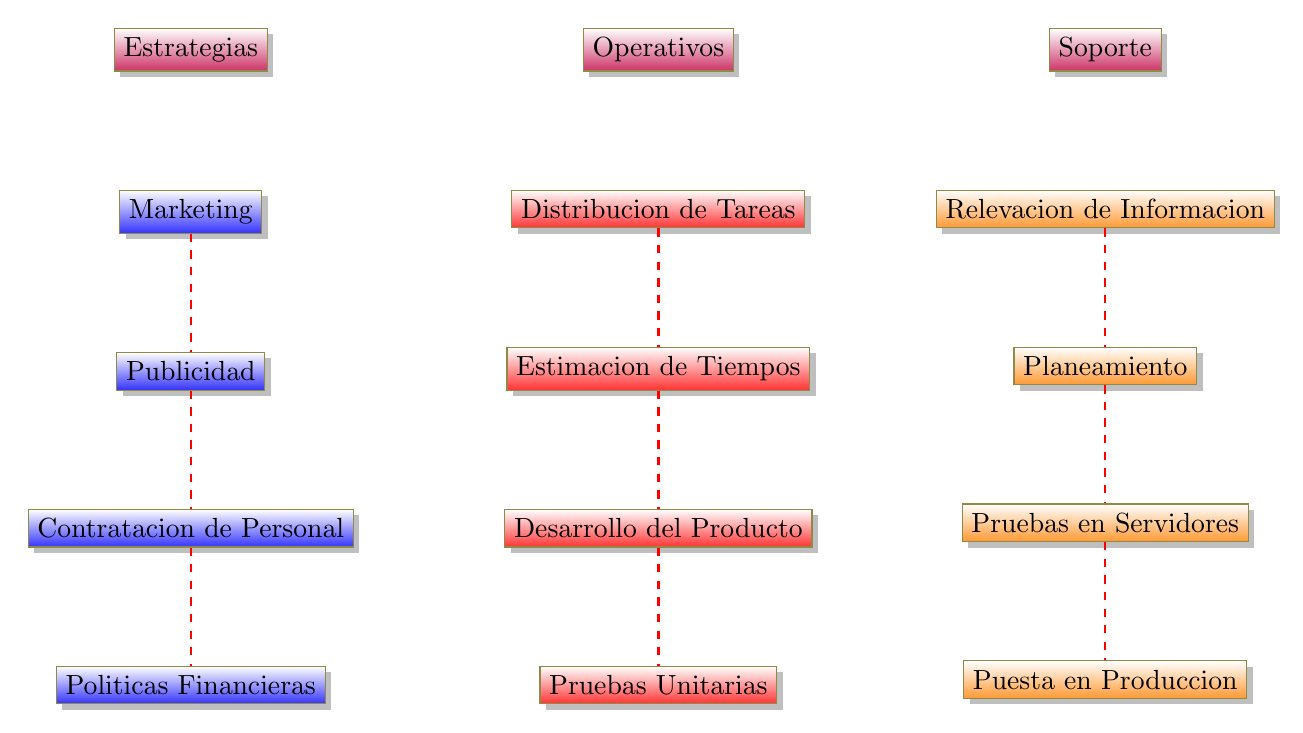
\begin{tikzpicture}[node distance=1.5cm, every edge/.style={link}]

% Titles
  \node[title]  (estr)                     {Estrategias};
  \node[title]  (oper) [right=4cm of estr] {Operativos};
  \node[title]  (supp) [right=4cm of oper] {Soporte};

% Strategic
  \node[strategic]  (node1) [below=of estr]  {Marketing};
  \node[strategic]  (node2) [below=of node1] {Publicidad};
  \node[strategic]  (node3) [below=of node2] {Contratacion de Personal};
  \node[strategic]  (node4) [below=of node3] {Politicas Financieras};

% Operative
  \node[operative]  (node5) [below=of oper]  {Distribucion de Tareas};
  \node[operative]  (node6) [below=of node5] {Estimacion de Tiempos};
  \node[operative]  (node7) [below=of node6] {Desarrollo del Producto};
  \node[operative]  (node8) [below=of node7] {Pruebas Unitarias};

% Support
  \node[support]    (node9)  [below=of supp]  {Relevacion de Informacion};
  \node[support]    (node10) [below=of node9]  {Planeamiento};
  \node[support]    (node11) [below=of node10] {Pruebas en Servidores};
  \node[support]    (node12) [below=of node11] {Puesta en Produccion};

  % Relations
  \draw[red, thick, dashed] (0,0) (node1)  -- (node2)  ;
  \draw[red, thick, dashed] (node2)  -- (node3)  ;
  \draw[red, thick, dashed] (node3)  -- (node4)  ;

  \draw[red, thick, dashed] (node5)  -- (node6)  ;
  \draw[red, thick, dashed] (node6)  -- (node7)  ;
  \draw[red, thick, dashed] (node7)  -- (node8)  ;

  \draw[red, thick, dashed] (node9)  -- (node10) ;
  \draw[red, thick, dashed] (node10) -- (node11) ;
  \draw[red, thick, dashed] (node11) -- (node12) ;

  \end{tikzpicture}
}


